\documentclass[12pt]{article}
\usepackage{hyperref}
\usepackage[authoryear, round,sort,comma,numbers]{natbib}
\usepackage{times}
\usepackage{color}
\usepackage{apalike}
\usepackage{graphicx}
\usepackage{authblk}
\usepackage{amsmath}



%\usepackage[maxbibnames=99]{biblatex}
%\usepackage{setspace}
%\usepackage{geometry}
\usepackage[font={sf,small}]{caption}
%\usepackage{setspace}
%\usepackage{geometry}
%\usepackage{hyperref}
%\hypersetup{
%    colorlinks,
%    citecolor=black,
%    filecolor=black,
%    linkcolor=black,
%    urlcolor=black
%}
%\geometry{letterpaper}

\usepackage{amssymb}
%\usepackage{epstopdf}
\usepackage{float}
%\DeclareGraphicsRule{.tif}{png}{.png}{`convert #1 `dirname #1`/`basename #1 .tif`.png}

\newcommand{\specialcell}[2][c]{%
	\begin{tabular}[#1]{@{}c@{}}#2\end{tabular}}
\setlength{\textheight}{9.3in}
\setlength{\textwidth}{7in}
\setlength{\footskip}{0.5in}
\setlength{\topmargin}{-0.5in}
\setlength{\headheight}{0.2in}
\setlength{\headsep}{0in}
\setlength{\parindent}{1pc}
\setlength{\oddsidemargin}{-0.25in}
\setlength{\evensidemargin}{-0.25in}
\renewcommand{\baselinestretch}{1.5}
%\renewcommand{\figurename}{Supplementary Figure}
\renewcommand{\thefigure}{S\arabic{figure}}
\renewcommand{\thetable}{S\arabic{table}}

\usepackage{changes}
\definechangesauthor[name={Siyu Wang}, color=red]{siyu}
\definechangesauthor[name={Bob}, color=blue]{bob}
\usepackage{blindtext}
\usepackage{titlesec}


\title{Supplementary Materials: Separating random and deterministic sources of computational noises in explore-exploit decisions}
\author[1,\textcurrency]{Siyu Wang}
\author[1,2,3]{Robert C. Wilson}


\affil[1]{Department of Psychology, University of Arizona, Tucson AZ, USA}
\affil[2]{Neuroscience and Physiological Sciences Graduate Interdisciplinary Program, University of
	Arizona, Tucson AZ, USA}
\affil[3]{Cognitive Science Program, University of Arizona, Tucson AZ, USA}
\affil[ \textcurrency]{Current Address: Laboratory of Neuropsychology, National Institute of Mental Health, National Institutes of Health, Bethesda MD, USA}
      
%\date{\today}

\begin{document}
	\maketitle
	\newpage
	\tableofcontents

	\section{Additional model-free analyses}
	\subsection{Replication of Figure 2 without excluding subjects}
	\begin{figure}[H]
		\begin{center}
			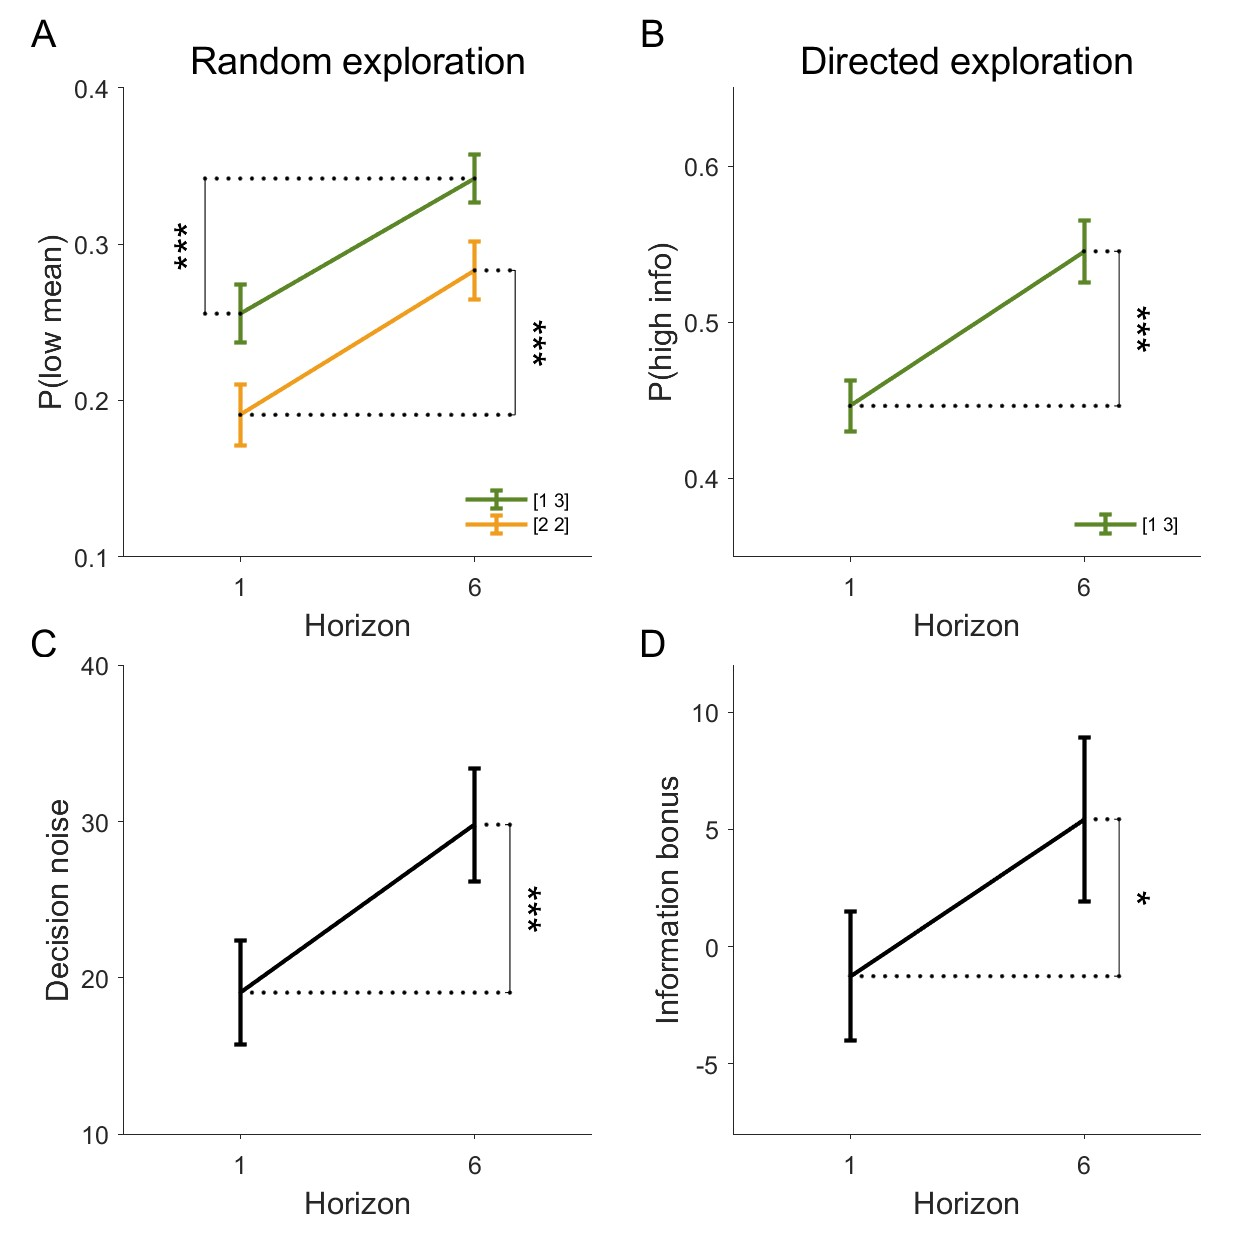
\includegraphics[width=\textwidth]{figures/RanDetNoise_modelfree__all.jpg}
			\caption{Replication of previous findings with data from all participants (i.e. no exclusions).  (A) model-free measure of behavioral variability, $p(\mbox{low mean})$, increases with horizon. (B) model-free measure of information seeking, $p(\mbox{high info})$, increases with horizon. (C) model-based measure of behavioral variability, decision noise $\sigma$, increases with horizon. (D) model-based measure of information seeking, information bonus $A$, increases with horizon.}
			\label{fig:s1}
		\end{center}
	\end{figure}
	\newpage

	\subsection{Replication of Figure 3 without excluding subjects}
	\begin{figure}[H]
		\begin{center}
			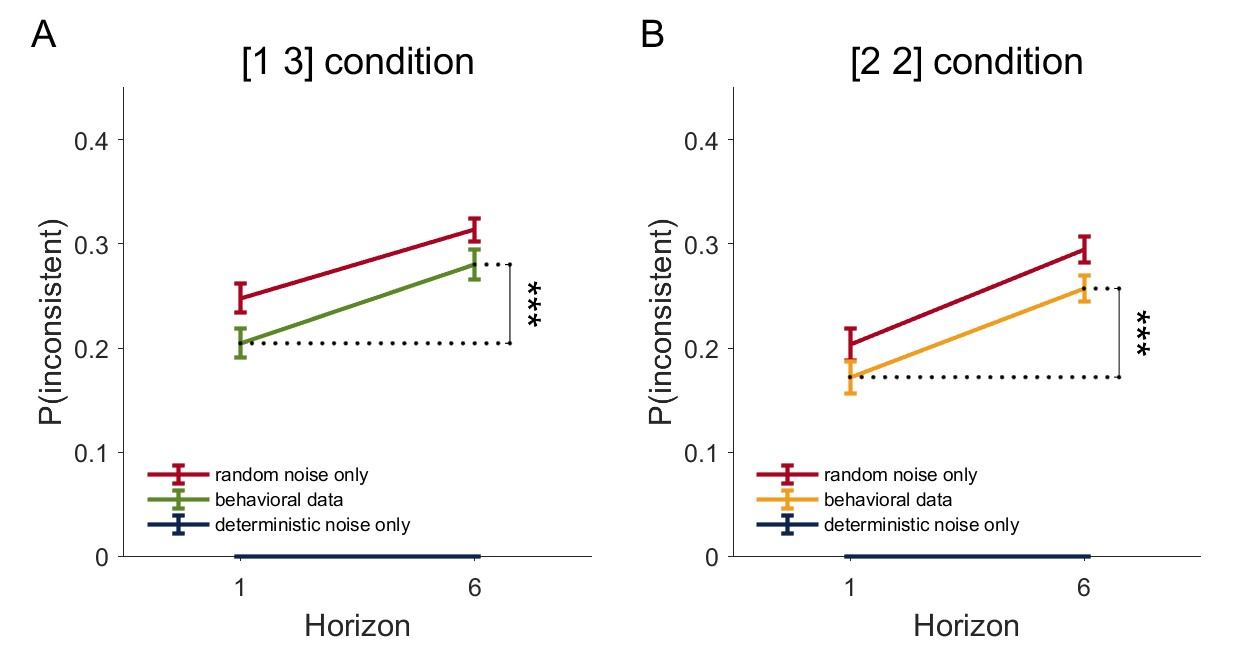
\includegraphics[width=\textwidth]{figures/RanDetNoise_pinconsistent__all.jpg}
			\caption{Model-free analysis with data from all participants (i.e. no exclusions) suggests that both deterministic and random noise contribute to the choice variability in random exploration. For both the [1 3] (A) and [2 2] (B) condition, people show greater choice inconsistency in horizon 6 than horizon 1. However, the extent to which their choices are inconsistent lies between what is predicted by purely deterministic and random noise, suggesting that both noise sources influence the decision.}
			\label{fig:s2}
		\end{center}
	\end{figure}

	\newpage

	\subsection{Model-free analysis with simulated choice from a pure random noise model}
	\begin{figure}[H]
	\begin{center}
		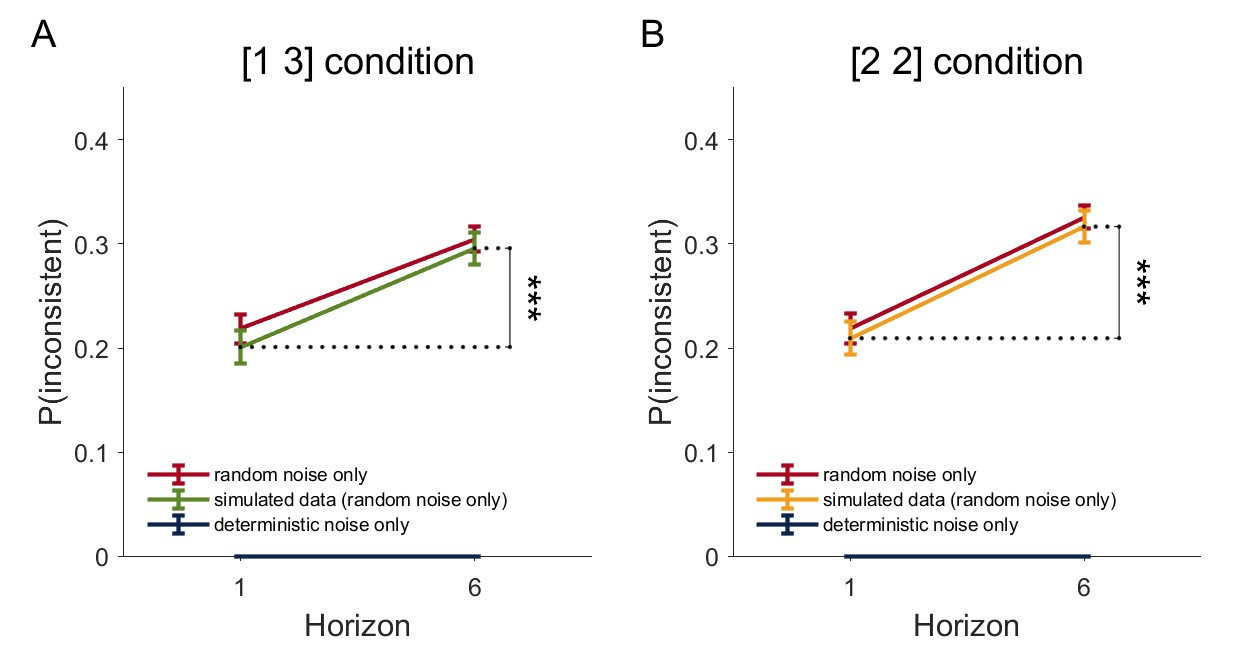
\includegraphics[width=\textwidth]{figures/RDBayes_pinconsistent_validation.jpg}
		\caption{Model-free analysis with simulated choices from a model that has only random noise validates our prediction of p(inconsistent) for pure random noise. The extent to which simulated choices are inconsistent completely overlaps with our pure random noise prediction(p $>$ 0.05). This suggests that when choice inconsistency lies below the pure random noise prediction indeed provides evidence that deterministic noise exists in random exploration (Figure 3).}
		\label{fig:s3}
	\end{center}
	\end{figure}
	\newpage
	\section{Model validation analyses}
	\subsection{Deterministic noise captures known deterministic processes excluded from the model}	
	We checked if our fitted deterministic noise could indeed capture unobserved deterministic process that was not accounted for by the decision model. We test this by leaving out one known deterministic process from the decision model, and ask if our method could recover that known deterministic process as deterministic noise. In particular, we fit a reduced version of our model that only considers reward and ignores the influence of uncertainty condition and spatial bias on explore-exploit decisions.  
	$$\Delta Q= \Delta R+n_{det}+n_{ran}$$
	Here, $\Delta Q, \Delta R, n_{det}, n_{ran}$ represent the same variables as in the full model (Equation 2 in the manuscript).	If deterministic noise in our model can indeed capture unobserved deterministic processes that's missed by the model, then we would expect to see a higher level of fitted deterministic noise in the reduced model compared to in the full model, whereas the level of random noise should remain unchanged. By comparing the	fitted posterior distributions over the group-level means of the deterministic and random noise parameters $\sigma_{det}$ and $\sigma_{ran}$, as expected, we observed an increase in deterministic noise and no change in random noise between the reduced and the full model (Figure \ref{fig:reducedmodel}). This suggests that our model is capable of detecting missing deterministic processes.
	
	\begin{figure}[H]
		\begin{center}
			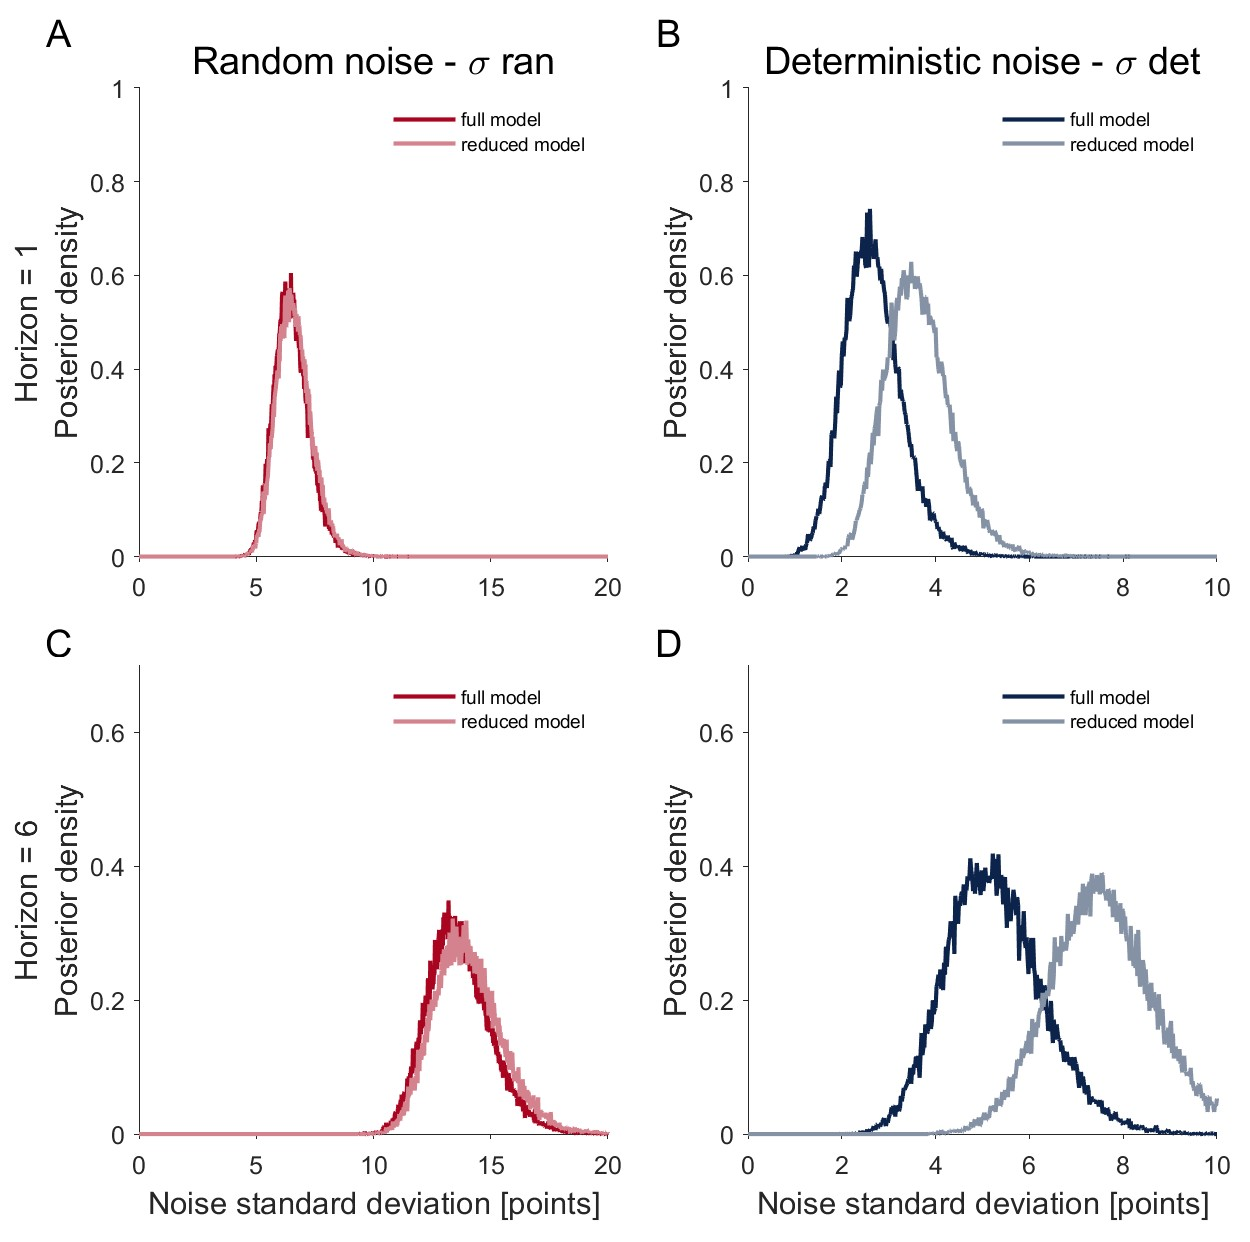
\includegraphics[width=\textwidth]{figures/RDBayes_reduced_model.jpg}
			\caption{Deterministic noise can recover known deterministic processes that's intentionally omitted by the model. In the reduced model where the deterministic effect of uncertainty condition is omitted from the model, deterministic noise is higher compared to the full model that accounts for the effect of uncertainty. Random noise remains unchanged between the two models.}
			\label{fig:reducedmodel}
		\end{center}
	\end{figure} 
	\newpage
	\subsection{Frequentist coverage analysis}	
	We next evaluated our hierarchical Bayesian analysis procedure using the `frequentist coverage analysis'. In the coverage analysis, we simulated choices with the fitted parameters from the Hierarchical Bayesian analysis, and then re-fit the model to the simulated choices to see whether we can recover the parameters (Figure \ref{fig:coverage}). The simulation and re-fitting was repeated for 200 times. Then we counted out of the 200 repetitions how many times the true parameter that we simulate the choices from lies in the fitted 95\% confidence interval (Figure \ref{fig:coverage2}). This ratio will be referred to as the coverage rate. If our model fitting is reliable, then the fitted confidence interval should cover the true parameter for more than 95\% of the simulations. For random noise, the coverage rate is 100\% for both horizon 1, horizon 6, and the horizon difference. For deterministic noise, the coverage rate is 66\% for horizon 1 and 69\% for horizon 6. By comparing the posterior distributions of parameters that were used to generate simulations and the posterior distribution of recovered parameters, it is clear that our model systematically underestimates deterministic noise (Figure \ref{fig:coverage},  \ref{fig:coverage2}). Despite the underestimation of deterministic noise in both horizons, we could still reliably detect the horizon changes of deterministic noise (coverage rate is 97\%). This is because the underestimation of deterministic noise is partially canceled out when the difference is taken between horizons. For random noise, our model fitting procedure yields a faithful recovery. However, there is a conceptual limitation. Because random noise is modeled as non-stimulus-driven noise, it can include both true stochastic random noise and possible deterministic noises which do not depend on the stimuli. Because of this, our random noise estimate provides an upper bound of true `random noise' induced by intrinsic stochastic processes in the brain.
	
	\begin{figure}[H]
		\begin{center}
			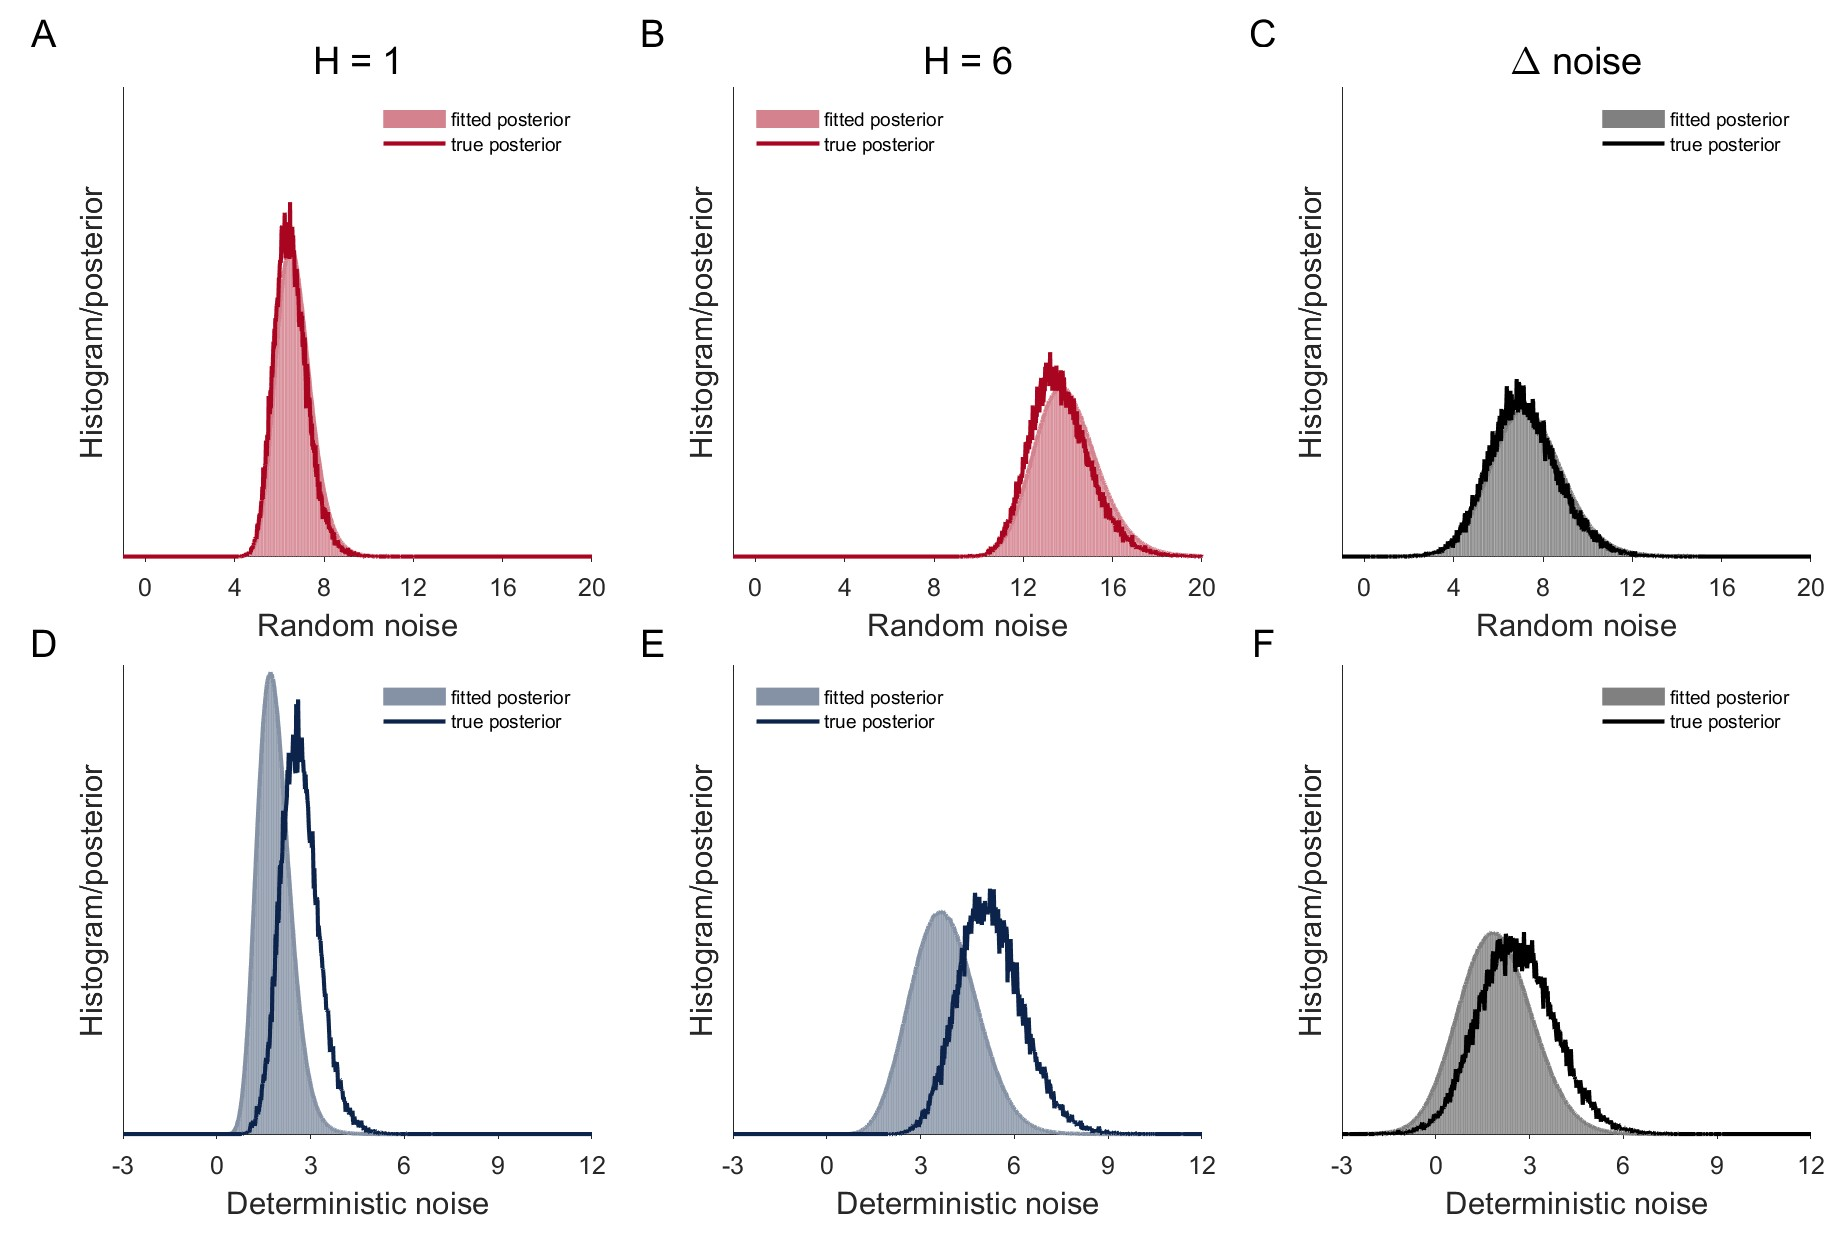
\includegraphics[width=1\textwidth]{figures/RDBayes_parameterrecovery_hyperprior_v2.jpg}
			\caption{Parameter recovery over the posterior distribution of random and deterministic noise standard deviations $\sigma_{det}$ and $\sigma_{ran}$. Solid lines are true posterior used to simulate choices. Lighter color shades represent the re-fitted posterior to the simulated choices. Our model fitting procedure faithfully recovers the non-stimulus-driven random noise (A, B), but systematically underestimates deterministic noise in both horizons (D, E). The horizon differences in random noise is also faithfully recovered (C). The horizon differences in deterministic noise is also underestimated but not significant (F).}
			\label{fig:coverage}
		\end{center}
	\end{figure} 
	
	\begin{figure}[H]
		\begin{center}
			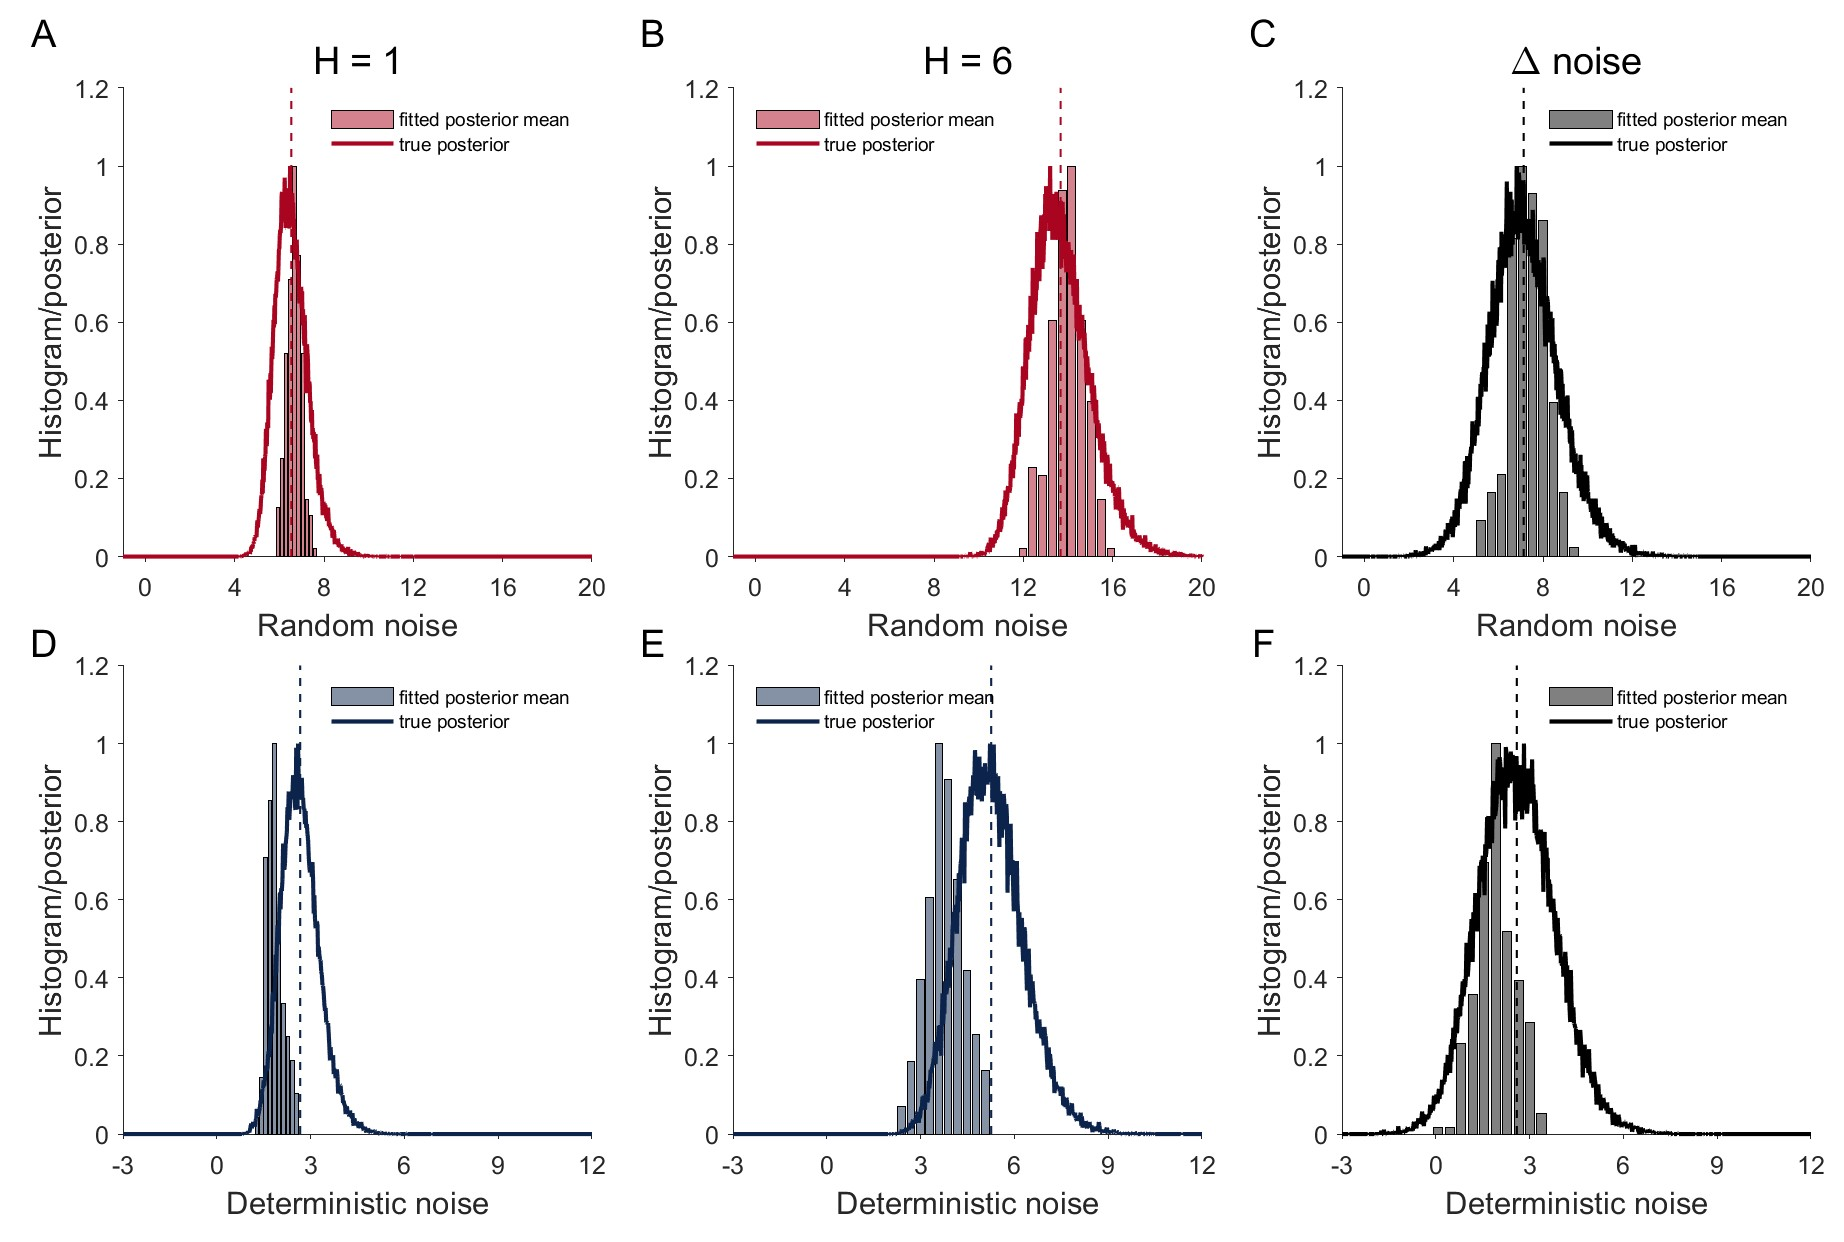
\includegraphics[width=1\textwidth]{figures/RDBayes_parameterrecovery_hyperprior.jpg}
			\caption{Parameter recovery over the mean estimates of random and deterministic noise standard deviations $\sigma_{det}$ and $\sigma_{ran}$. Solid lines are true posterior used to simulate choices, dashed black line is the mean of the true posterior. Histograms represent the mean estimates of the respective parameters in the refitting to the simulated data. (A) and (B) are random noise at H = 1 and H = 6, respectively. (C) is the random noise differences between horizons. (D) and (E) are deterministic noise at H = 1 and H = 6, respectively. (F) is the deterministic noise differences between horizons.}
			\label{fig:coverage2}
		\end{center}
	\end{figure}

	\newpage
	\subsection{Parameter recovery of the subject-level parameter fits}
	Next, we tested the ability of our model fitting procedure to recovery parameters from simulated data at the subject level (Figure \ref{fig:paramrecover_session}, \ref{fig:paramrecover_sub}). The correlations between the true vs fitted parameters are significant across participants for all parameters (p $<$ 0.001). The strength of correlation between simulated and fit values are strong for both deterministic noise (R $>$ 0.8, Figure \ref{fig:paramrecover_sub}) and random noise (R $>$ 0.9, Figure \ref{fig:paramrecover_sub}). Despite the strong inter-subject correlations, we again observed a systematic underestimation of $\sigma_{det}$ (Figure \ref{fig:paramrecover_session}, \ref{fig:paramrecover_sub}).
	
	Overall, we are able to detect both deterministic and random noises using our model to a satisfactory extent. Our model provides a lower bound for deterministic noise and an upper bound for random noise. In addition, We see better parameter recovery for random noise than deterministic noise. This is likely because we effectively have half as many trials for deterministic noise. In particular, while we generate two samples of random noise for each repeated game pair, we only generate one sample of deterministic noise, which by definition is the same in both of the repeated games. 
	
	\begin{figure}[hp]
		\begin{center}
			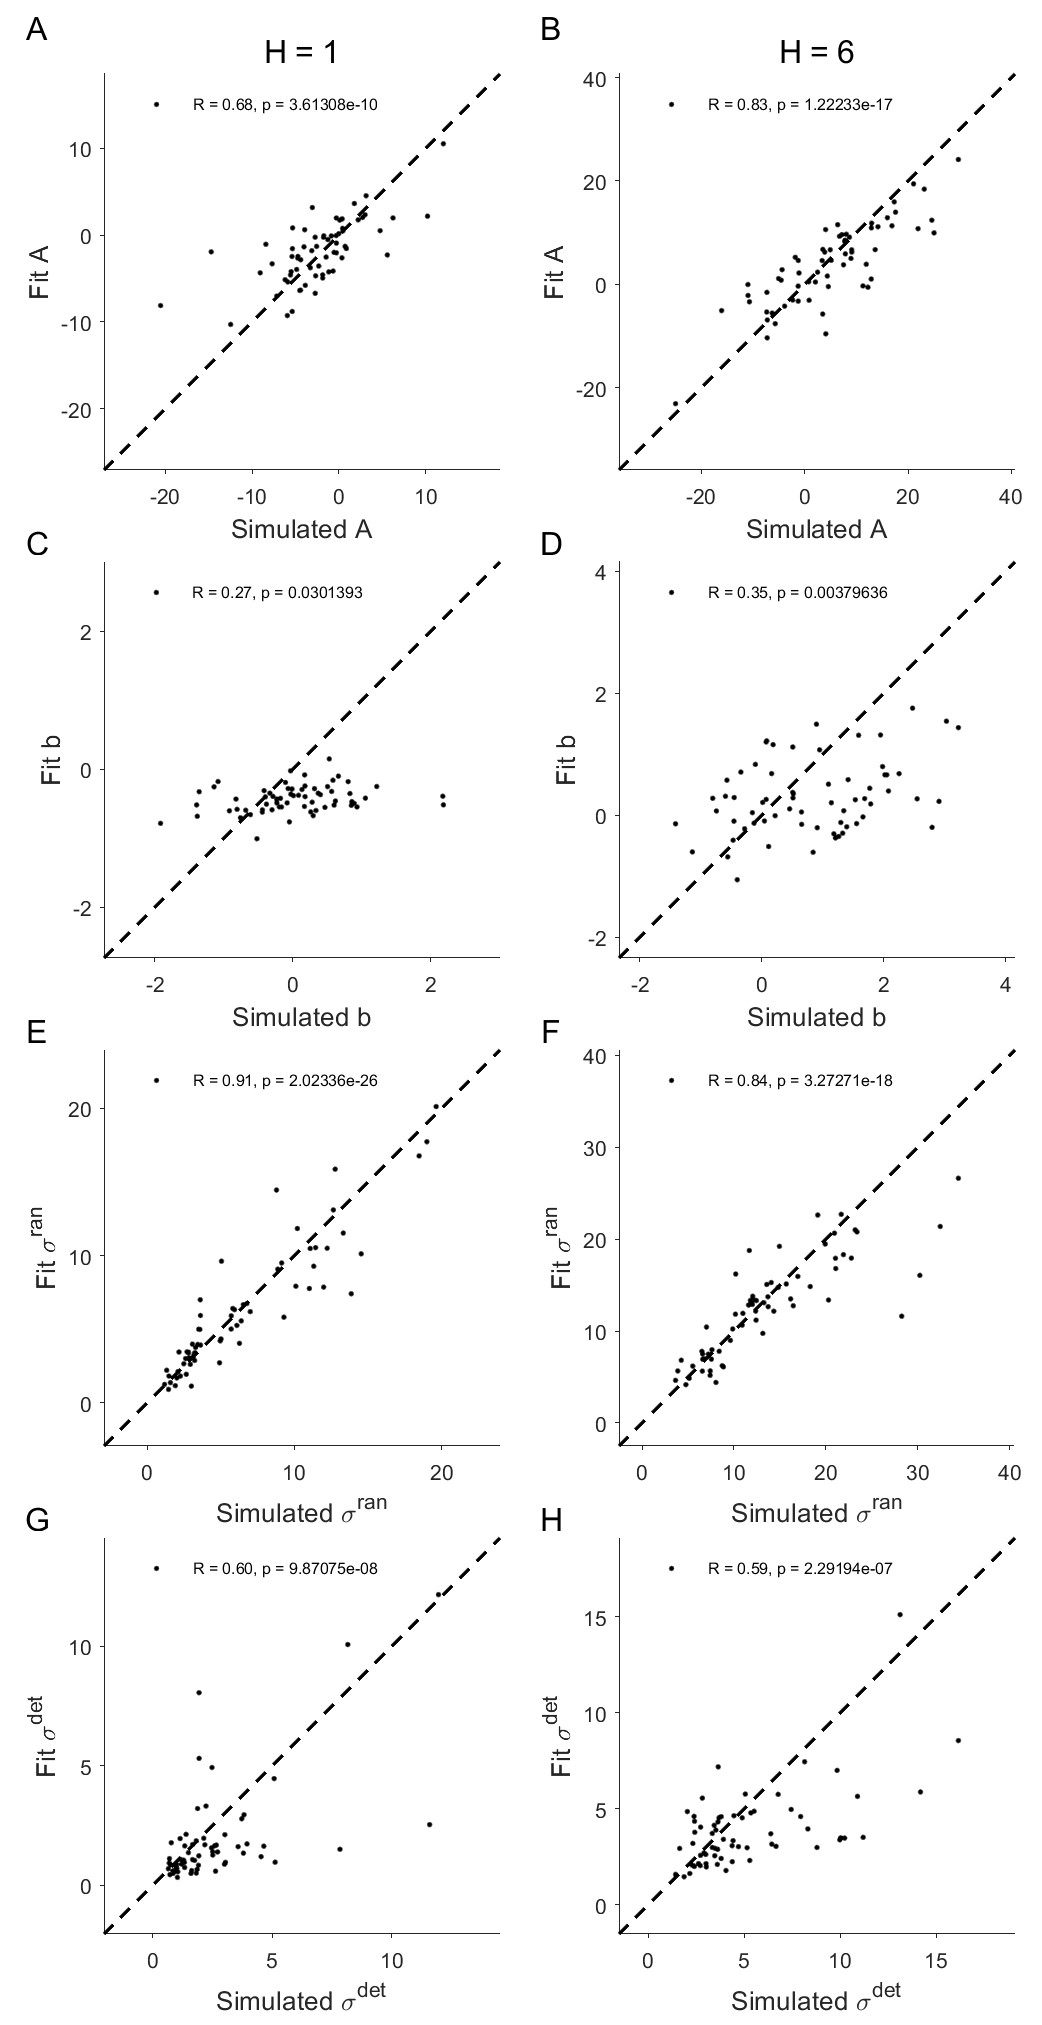
\includegraphics[width=0.65\textwidth]{figures/RDBayes_parameterrecovery_subject_examplesession.jpg}
			\caption{Parameter recovery over the subject-level means of information bonus, $A$, spatial bias, $b$, random noise standard deviation, $\sigma_{ran}$, and deterministic noise standard deviation, $\sigma_{det}$, for horizon 1 (left column) and horizon 6 (right column) games.}
			\label{fig:paramrecover_session}
		\end{center}
	\end{figure} 

	\begin{figure}[hp]
		\begin{center}
			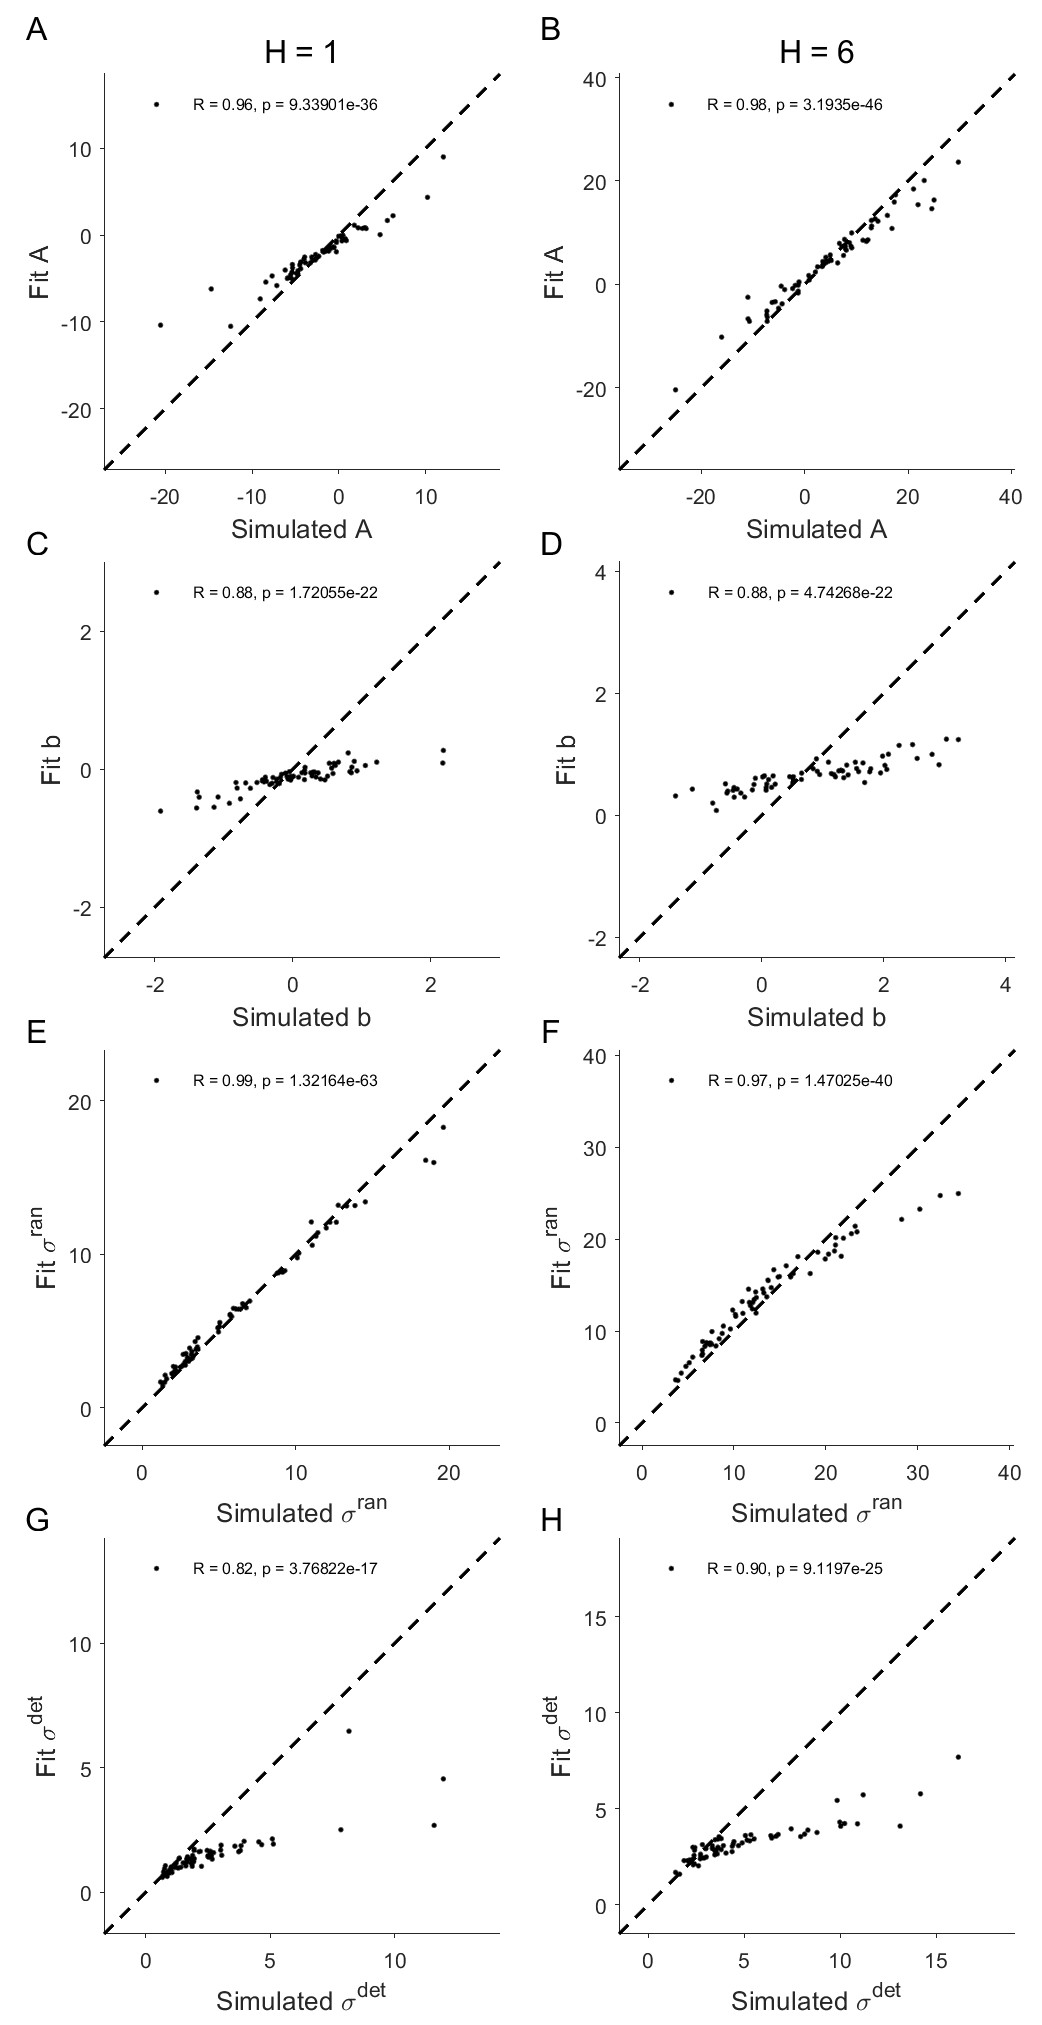
\includegraphics[width=0.65\textwidth]{figures/RDBayes_parameterrecovery_subject.jpg}
			\caption{Same as Figure \ref{fig:paramrecover_session}, except that the recovered parameters were averaged across 200 repetitions and then compared to the original parameters.}
			\label{fig:paramrecover_sub}
		\end{center}
	\end{figure} 
	
	
	\newpage	
	\subsection{Parameter recovery over a bigger range of arbitrary combinations of deterministic and random noises \label{gridrecovery}}
	
	%Parameter recovery is good (in terms of) for all parameters apart from the bias in short horizon condition, which is likely due to this parameter being so close to zero (Figure \ref{fig:pararecover1} Panel C). The recovery for the noise parameters, $\sigma_{det}$ and $\sigma_{ran}$, is slightly better for horizon 1 than horizon 6.
	
	Lastly, in addition to testing how our model performs in parameter ranges around the actual fitted parameters, we tested the limitations of our models in arbitrary combinations of random vs deterministic noises. All combinations of random and deterministic noises with $0 \le \sigma_{det} \le 10$ and $0 \le \sigma_{ran} \le 10$ were tested. In a special case, we evaluated how our model performs when there is only random noise or only deterministic noise (Figure \ref{fig:puredetran}). In the simulation with fully deterministic noise and 0 random noise, our model successfully recovered both random and deterministic noise (Figure \ref{fig:puredetran} C, D), however in the simulation with fully random noise and 0 deterministic noise, although our model successfully recovered random noise, some small proportion of deterministic noise was falsely detected when they should instead be 0 (Figure \ref{fig:puredetran} A, B). However, this phenomenon only exists when the true deterministic noise is 0, once the true deterministic noise is greater than 1, we don't observe this obvious inflation of deterministic noise anymore (Figure \ref{fig:gridall}). Apart from this, our model did a fairly good job in recovering all combinations of random and deterministic noises (Figure \ref{fig:gridall}).
	
	%This is because it requires more trials to recover larger values of $\sigma_{det}$ and $\sigma_{ran}$, so with the same number of choices it is harder to recover overall larger noise variances in horizon 6. 
	
	\begin{figure}[H]
		\begin{center}
			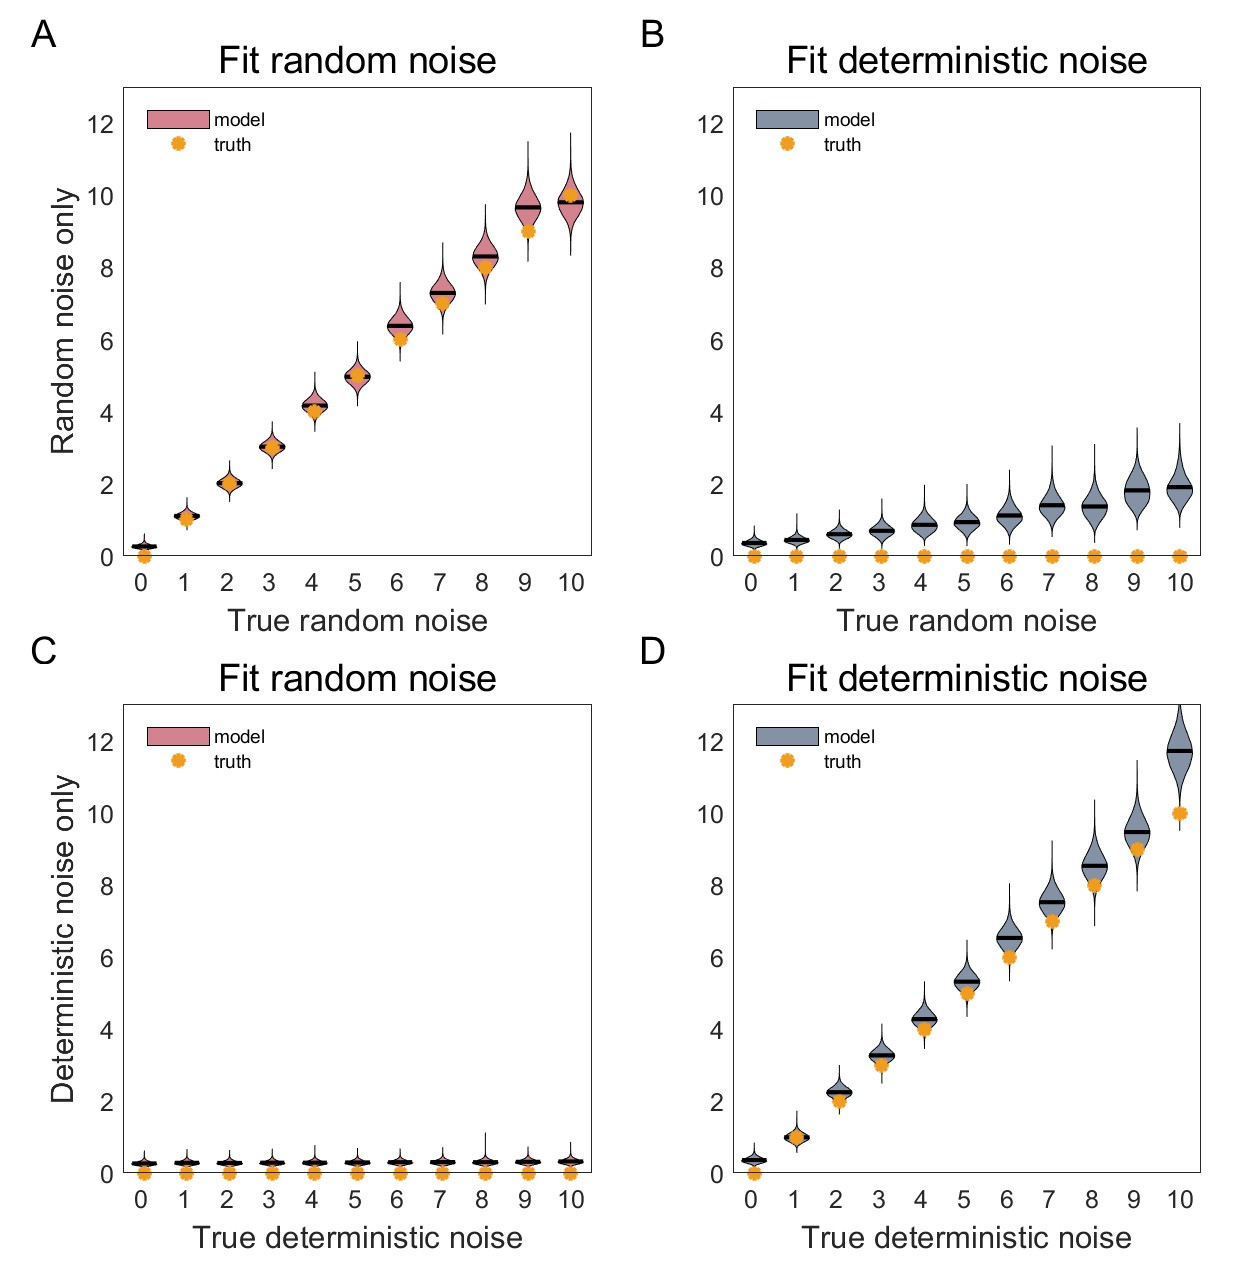
\includegraphics[width=0.7\textwidth]{figures/RDBayes_parameterrecovery_grid_pureRanDet.jpg}
			\caption{Parameter recovery over the posterior of random noise standard deviation, $\sigma_{ran}$, and deterministic noise standard deviation, $\sigma_{det}$, for purely random noise (top row) and purely deterministic noise (bottom row) games. 
			}
			\label{fig:puredetran}
		\end{center}
	\end{figure} 

	\begin{figure}[hp]
		\begin{center}
			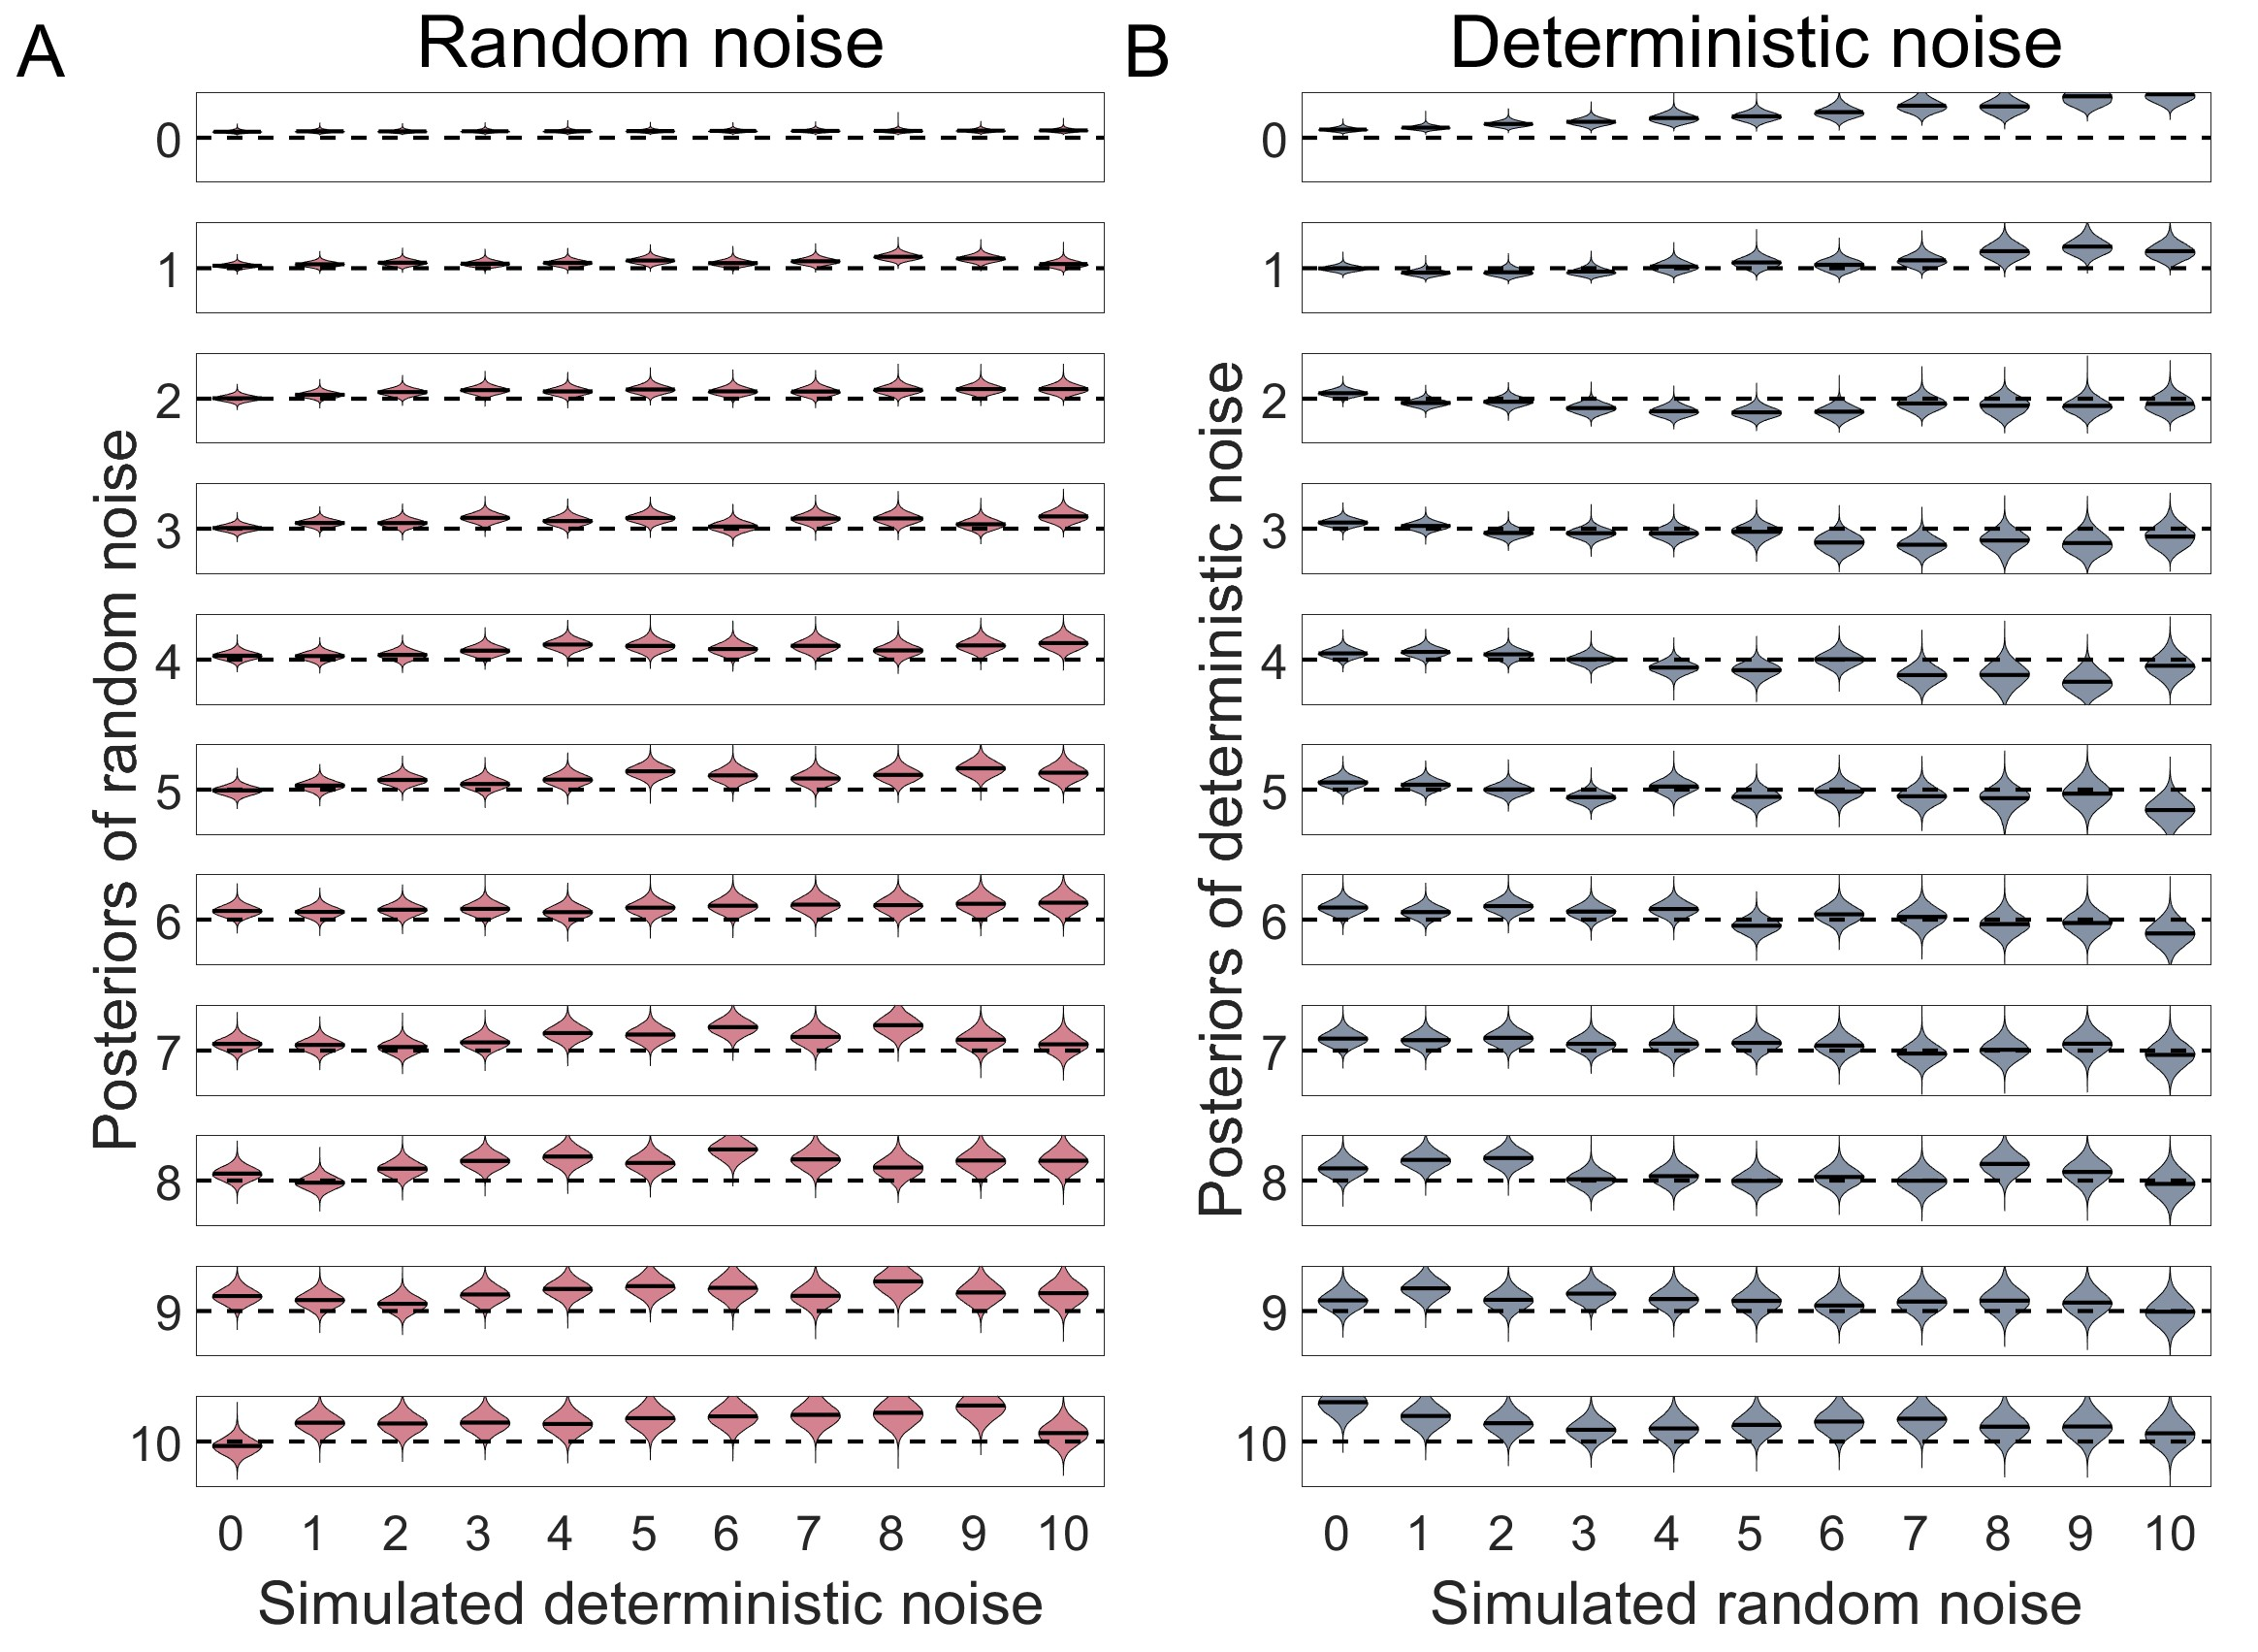
\includegraphics[width=1\textwidth]{figures/RDBayes_parameterrecovery_gridsimu_all.jpg}
			\caption{Parameter recovery on arbitrary combinations of random and deterministic noises. A. Recovered posterior distributions of random noise. B. Recovered posterior distributions of deterministic noise. For both A and B, from the top row to the bottom row, the true noise standard deviation that is used in the simulations go from 0 to 10. The y limit of each panel is 4 (+/- 2 from the true value). Our model did a relatively good job in recovering all combinations of deterministic and random noises.}
			\label{fig:gridall}
		\end{center}
	\end{figure} 
	
	\section{Additional model-based analyses}
	\subsection{Replication of Figure 5 without excluding subjects}
	\begin{figure}[H]
		\begin{center}
			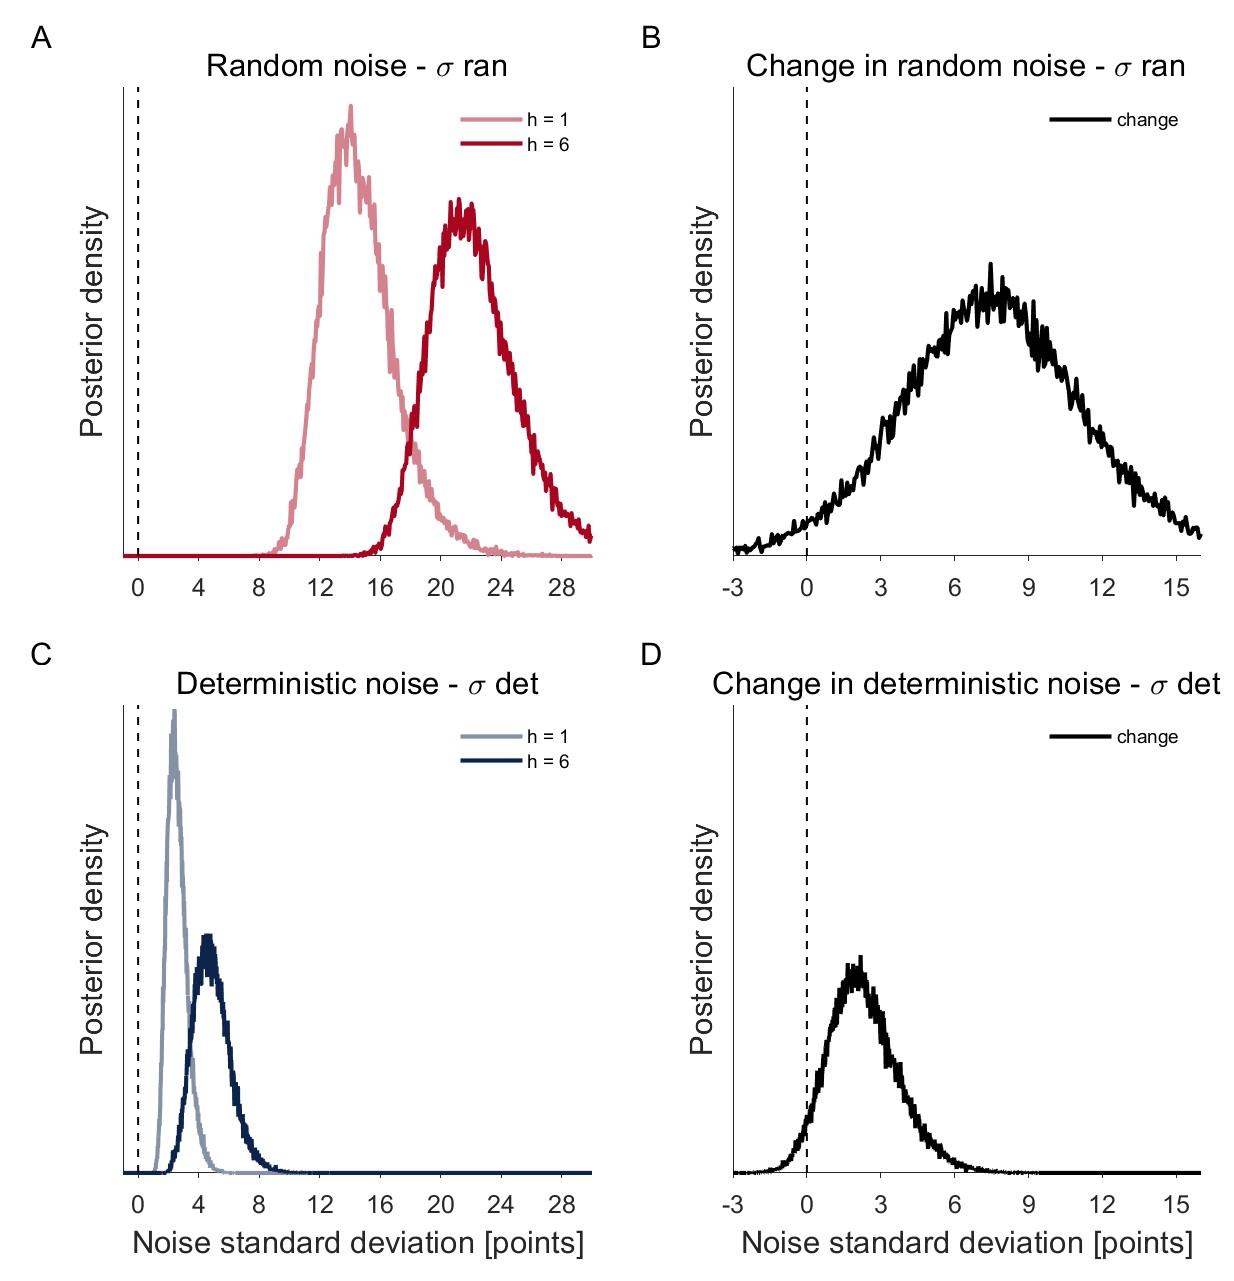
\includegraphics[width=0.7\textwidth]{figures/RDBayes_hyperprior__all.jpg}
			\caption{Model based analysis with data from all participants (i.e. no exclusions) showing the posterior distributions over the group-level mean of the standard deviations of  random and deterministic noise. Both random (A, B) and deterministic (C,D) noises are nonzero (A, C) and change with horizon (B, D).  However, random noise has both a greater magnitude overall (A, C) and a greater change with horizon (B, D) than deterministic noise.}
			\label{fig:s8}
		\end{center}
	\end{figure}
	\newpage
	\subsection{Alternative models: variations of the two-noise model}
	To check whether all aspects of the model were necessary to reproduce the qualitative pattern of findings, we also built and fit five additional versions of the model. These models varied in whether deterministic and random noise are present or not and whether either types of noise is dependent on horizon. Specifically, we tested the following 6 models (Note that the $\sigma^{ran}_{horizon},\sigma^{det}_{horizon}$ model is our original full model).
	
	\begin{table}[h]
		\small
		\centering
		\begin{tabular}{|c|c|c|}
			\hline
			Model & Deterministic noise & Random noise \\
			\hline
			$\sigma^{ran}_{horizon},\sigma^{det}_{horizon}$  & Horizon dependent & Horizon dependent\\
			\hline
			$\sigma^{ran}_{horizon},\sigma^{det}_{}$ & Fixed & Horizon dependent\\
			\hline
			$\sigma^{ran}_{},\sigma^{det}_{horizon}$ & Horizon dependent & Fixed\\
			\hline
			$\sigma^{ran}_{},\sigma^{det}_{}$ & Fixed & Fixed\\
			\hline
			$\sigma^{ran}_{horizon}$ & Horizon dependent & None\\
			\hline
			$\sigma^{det}_{horizon}$ & None & Horizon dependent\\
			\hline
		\end{tabular}
		\caption{Variants of the model.}
		\label{tab:models}	
	\end{table}

	The posterior distributions over the group-level means of the deterministic and random noise standard deviation $\sigma_{det}$ and $\sigma_{ran}$ (when they exist) in these model variants are shown in Figure \ref{fig:sixmodels}. 
	
	We again simulated choices using fitted parameters from these models and repeated the model-free analysis on the simulated data. As shown in Figure \ref{fig:posteriorcheck6models}, only one of these alternative models, where random noise is horizon dependent but deterministic noise is not, can capture the full qualitative pattern of behavior. However, the quantitative fit to the data is not as good (Figure \ref{fig:posteriorcheck6models}).% SIYU says: they actually look quite similar, without horizon dependent deterministic noise, the fixed det noise model is only marginally worse on p(inconsistent) in [2 2] condition, as it overlaps with the pure random noise line more.
	
	
	\begin{figure}[hp]
		\begin{center}
			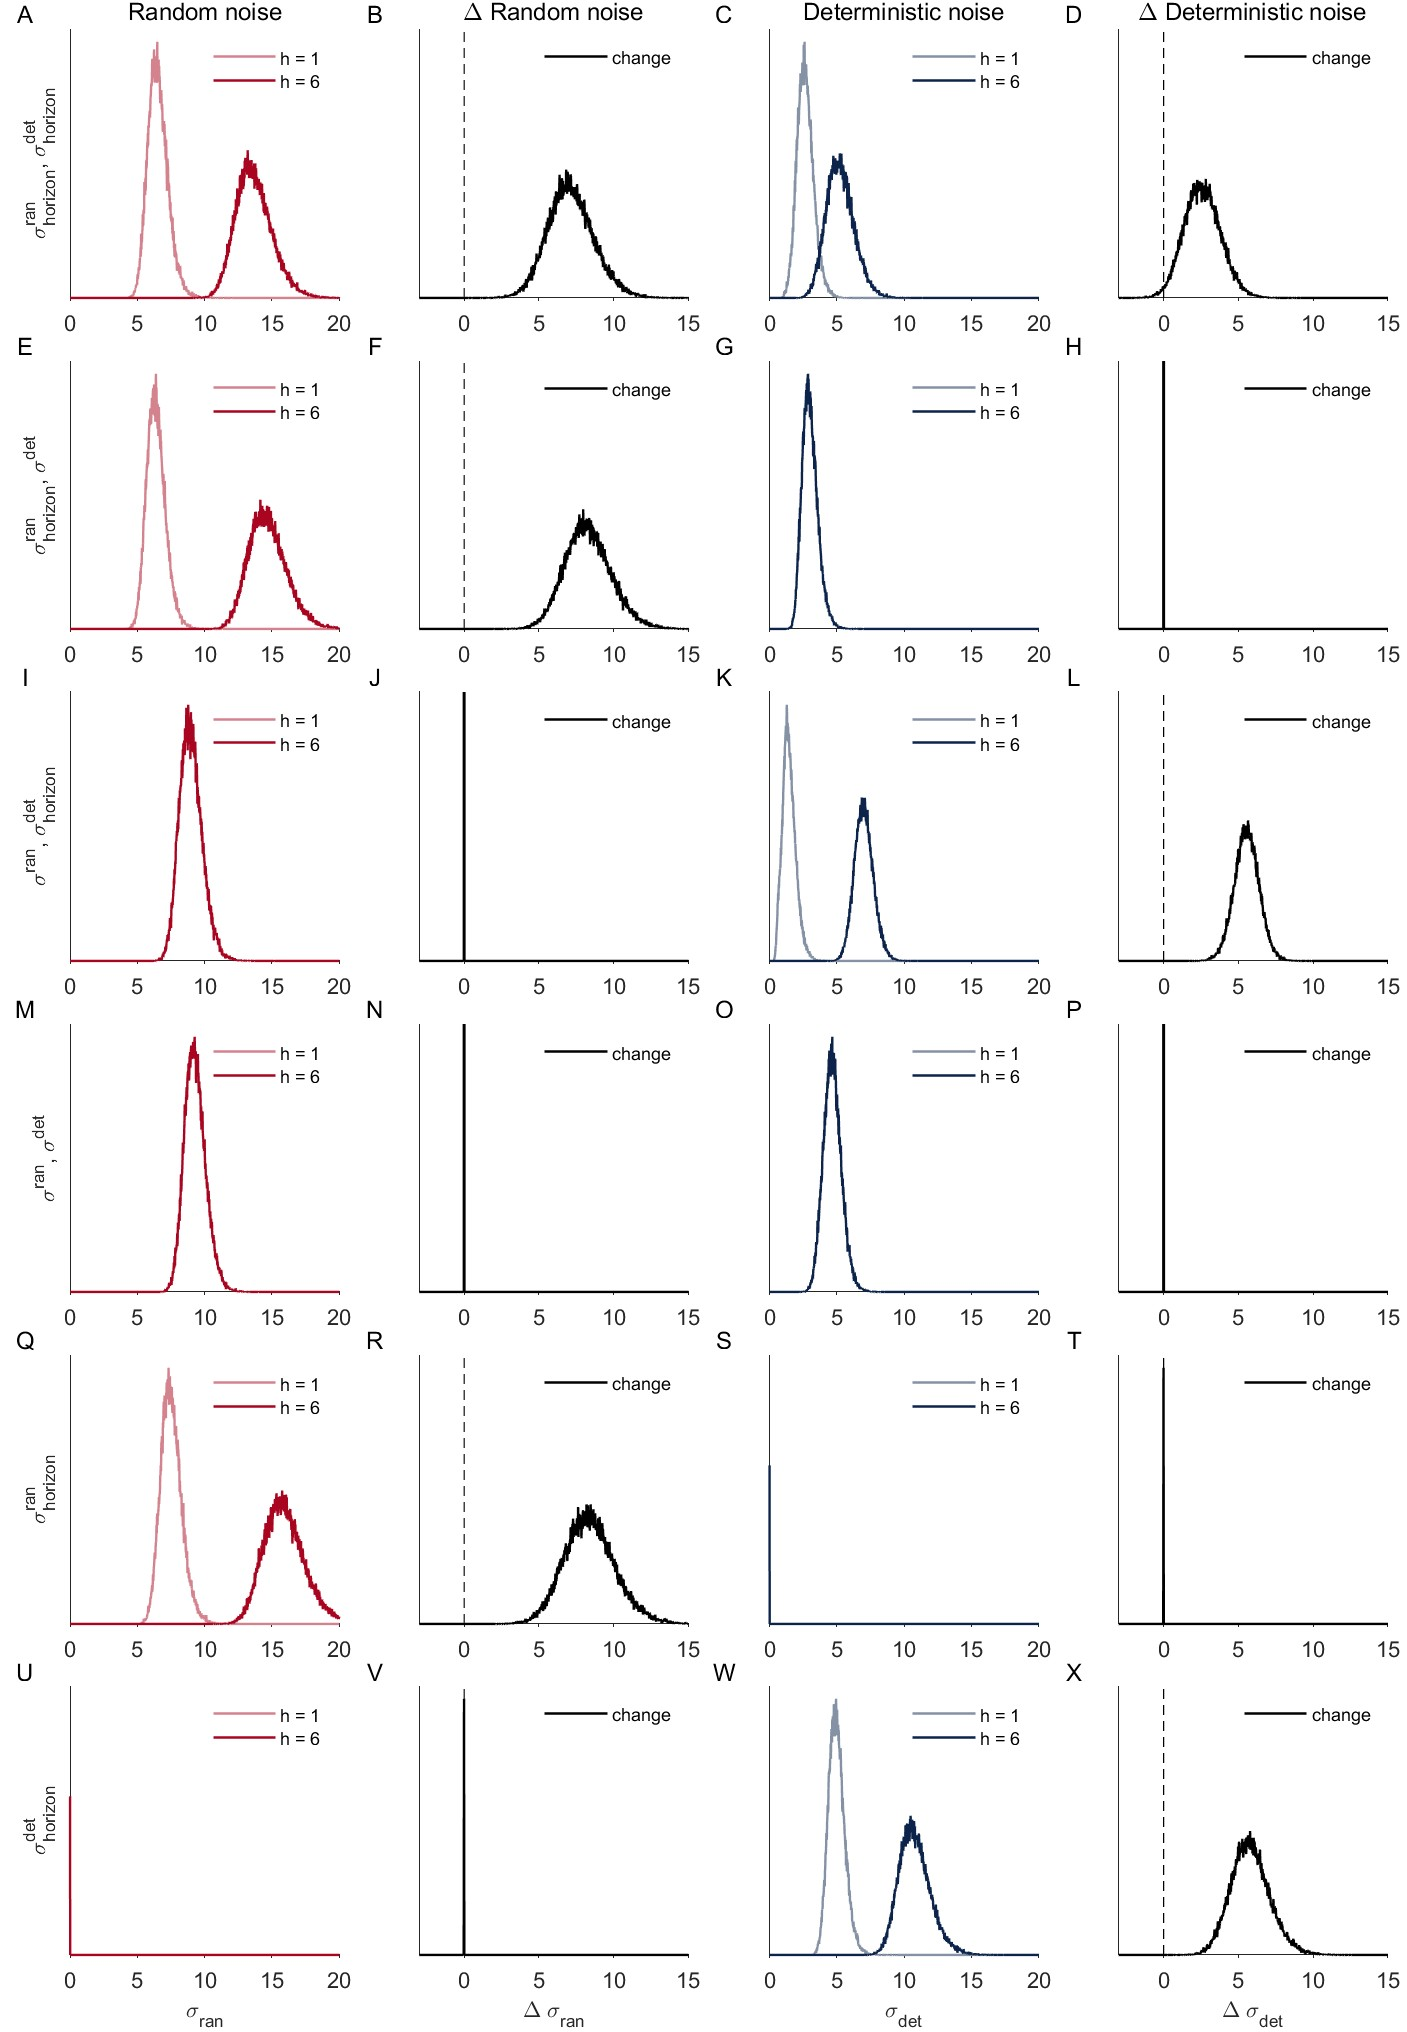
\includegraphics[width=0.8\textwidth]{figures/RDBayes_2noise_hyperpriors_6model.jpg}
			\caption{Model based analysis with alternative models. Each row is one model. These models varied in whether deterministic $\sigma^{det}$ and random noise $\sigma^{ran}$ are present or not and whether either types of noise is dependent on horizon (subscript denotes the dependence on horizon). }
			\label{fig:sixmodels}
		\end{center}
	\end{figure}

	\begin{figure}[hp]
		\begin{center}
			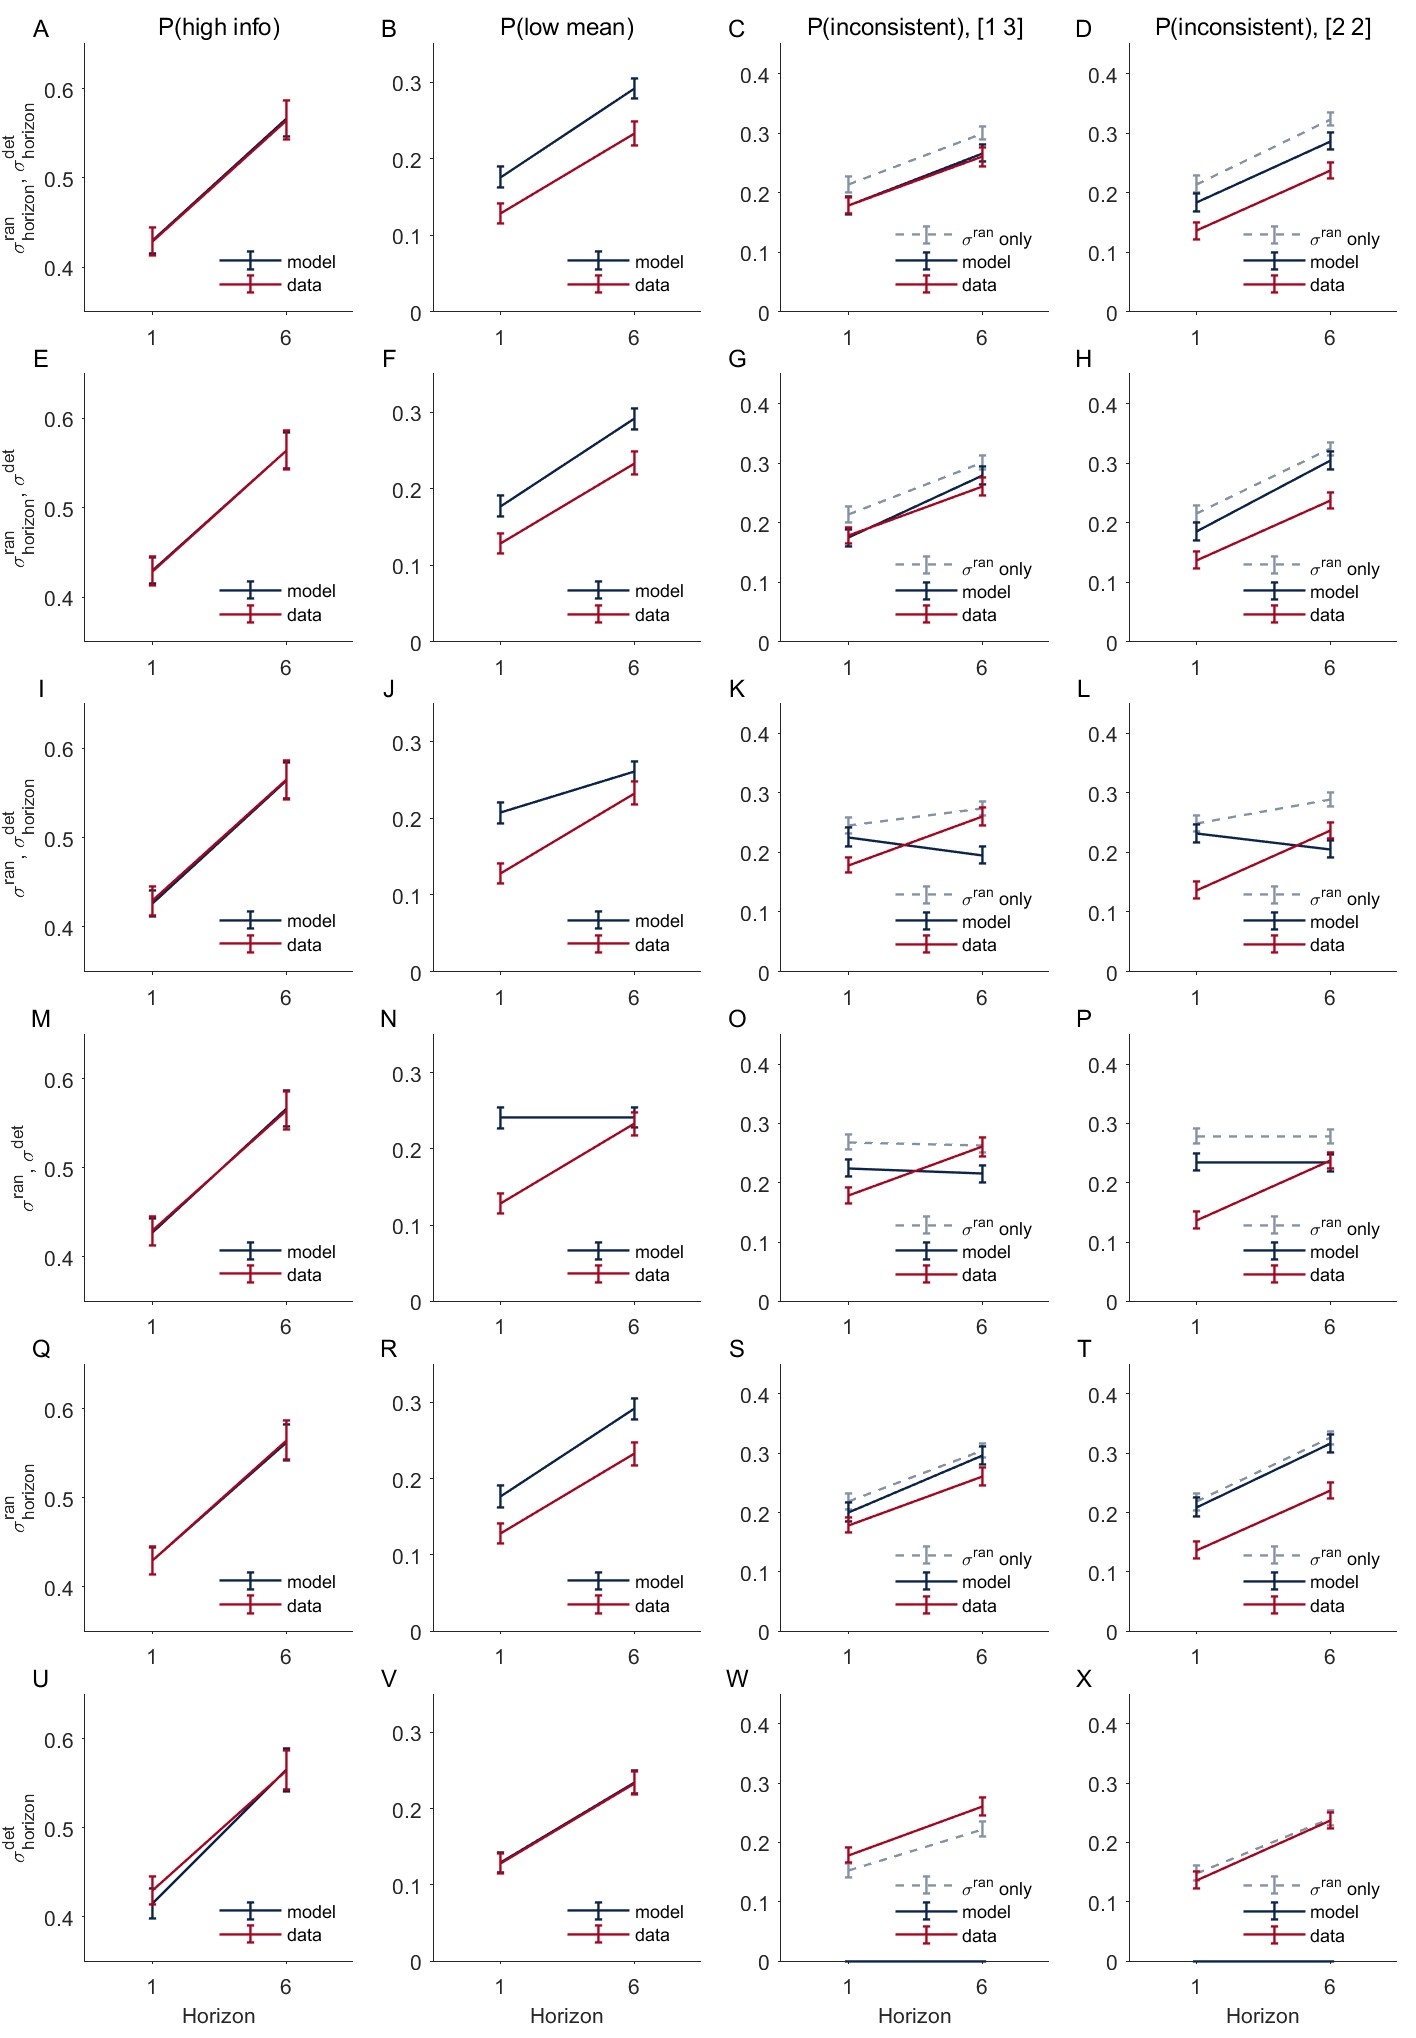
\includegraphics[width=0.8\textwidth]{figures/RDBayes_2noise_6modelcomparison.jpg}
			\caption{
				Model comparison. A-D. both deterministic and random noise are horizon dependent, E-H. only random noise is horizon dependent, I-L. only deterministic noise is horizon dependent, M-P. neither random nor deterministic noise is horizon dependent, Q-T. only deterministic noise is assumed to be present, U-X. only random noise is assumed to be present.}
			\label{fig:posteriorcheck6models}
		\end{center}
	\end{figure}
	

	Moreover, we examined if our model can indeed qualitatively capture whether deterministic and random noise are present or not and whether either types of noise is dependent on horizon. To test this, we simulated choices from each of the 6 models, and then fit the simulated choices with our original full model. The simulation was repeated 50 times for each model. Indeed, we showed that our model can capture both the existence of random and deterministic noise, and whether each noise changes with horizon condition (Figure \ref{fig:6model}), with only one exception that our model falsely detected a small fraction of deterministic noise when no deterministic noise was present (Figure \ref{fig:6model}). This phenomenon was also examined and discussed in the section \ref{gridrecovery} above.
	
	\begin{figure}[H]
		\begin{center}
			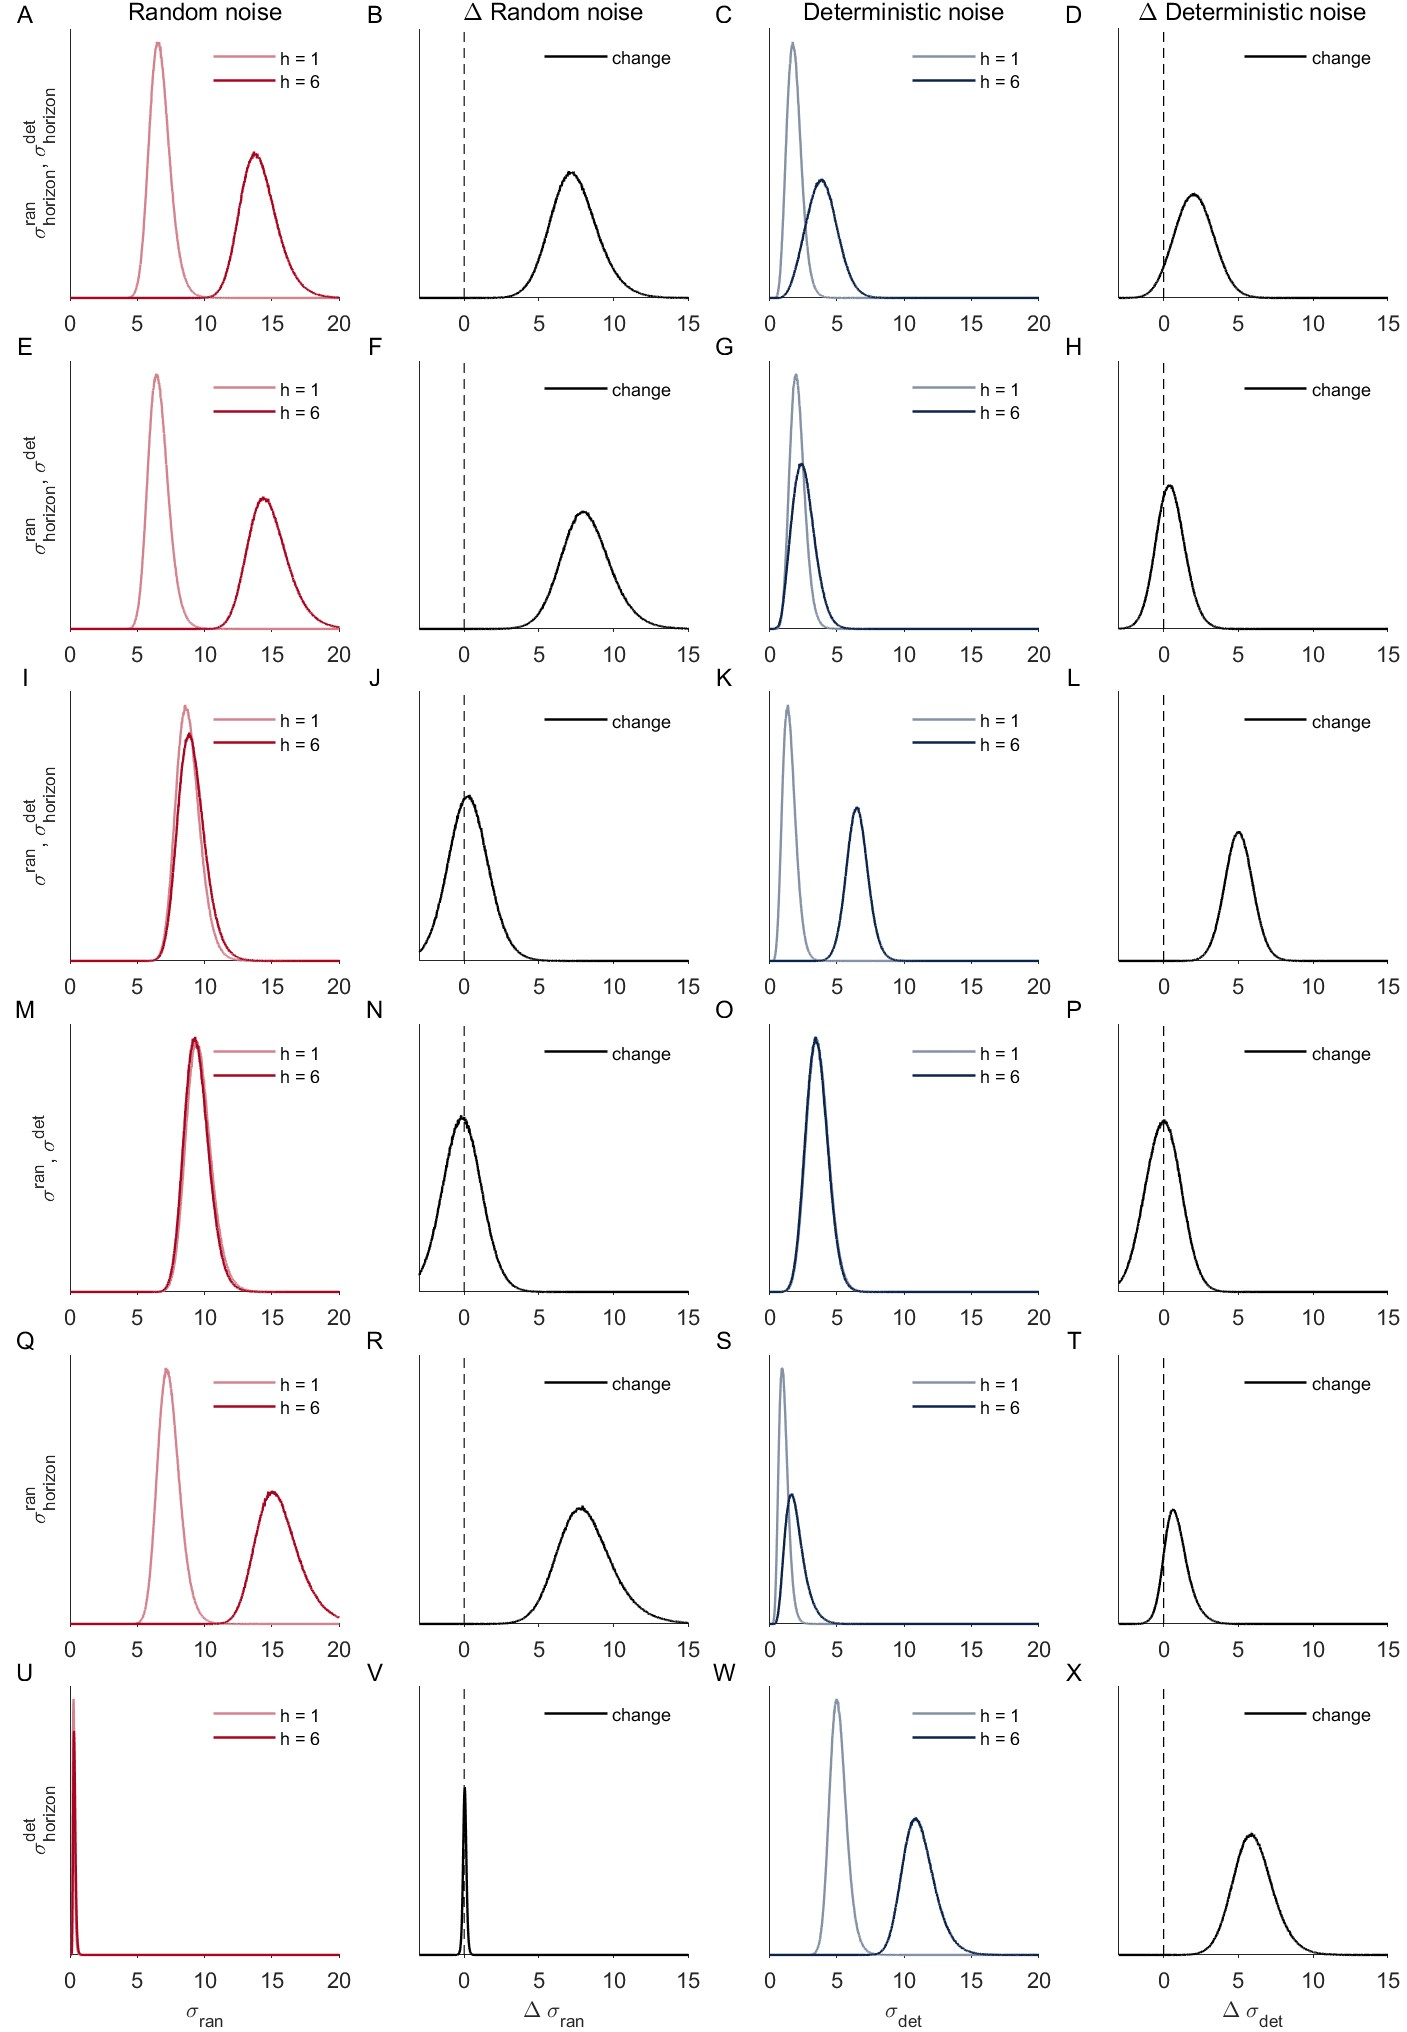
\includegraphics[width=0.8\textwidth]{figures/RDBayes_2noise_hyperprior_6model_recovery.jpg}
			\caption{
				Our model qualitatively captures whether deterministic and random noise are present or not and whether either types of noise is dependent on horizon. A-D. both deterministic and random noise are horizon dependent, E-H. only random noise is horizon dependent, I-L. only deterministic noise is horizon dependent, M-P. neither random nor deterministic noise is horizon dependent, Q-T. only deterministic noise is assumed to be present, U-X. only random noise is assumed to be present.}
			\label{fig:6model}
		\end{center}
	\end{figure}
\end{document}
